
%{{第三十五回}}{第三十五回}}

\chapter{白玉钏亲尝莲叶羹 黄金莺巧结梅花络}\label{part0039_split_000.htmlux5cux23calibre_pb_0}

{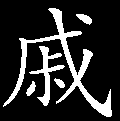
\includegraphics[width=3mm]{../Images/00005}情因相爱反相伤,何事人多不揣量。黛玉徘徊还自苦,莲羹甘受使儿狂。}

话说宝钗分明听见林黛玉刻薄他,因记挂着母亲哥哥,并不回头,一径去了。这里林黛玉还自立于花阴之下,远远的却向怡红院内望着,只见李宫裁、迎春、探春、惜春并各项人等都向怡红院内去过之后,一起一起的散尽了,只不见凤姐儿来,心里自己盘算道:``如何他不来瞧宝玉?便是有事缠住了,他必定也是要来打个花胡哨,讨老太太和太太的好儿才是。今儿这早晚不来,必有原故。''一面猜疑,一面抬头再看时,只见花花簇簇一群人又向怡红院内来了。定睛看时,只见贾母搭着凤姐儿的手,后头邢夫人王夫人跟着周姨娘并丫鬟媳妇等人都进院去了。

黛玉看了不觉点头,想起有父母的人的好处来,早又泪珠满面。少顷,只见宝钗薛姨妈等也进去了。忽见紫鹃从背后走来,说道:``姑娘吃药去罢,开水又冷了。''黛玉道:``你到底要怎么样?只是催,我吃不吃,管你什么相干!''紫鹃笑道:``咳嗽的才好了些,又不吃药了。如今虽然是五月里,{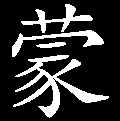
\includegraphics[width=3mm]{../Images/00006}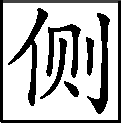
\includegraphics[width=3mm]{../Images/00011}\footnotesize \kaishu 闺中相怜之情,令人羡慕之至。}天气热,到底也该还小心些。大清早起,在这个潮地方站了半日,也该回去歇息歇息了。''一句话提醒了黛玉,方觉得有点腿酸,呆了半日,方慢慢的扶着紫鹃,回潇湘馆来。

一进院门,只见满地下竹影参差,苔痕浓淡,不觉又想起《西厢记》中所云``幽僻处可有人行,点苍苔白露泠泠''二句来,因暗暗的叹道:``双文,双文,诚为命薄人矣。然你虽命薄,尚有孀母弱弟;今日林黛玉之命薄,一并连孀母弱弟俱无。古人云`佳人命薄',然我又非佳人,何命薄胜于双文哉!''一面想,一面只管走,不防廊上的鹦哥见林黛玉来了,``嘎''的一声扑了下来,倒吓了一跳,因说道:``作死的,又扇了我一头灰。''那鹦哥仍飞上架去,便叫:``雪雁,快掀帘子,姑娘来了。''黛玉便止住步,以手扣架道:``添了食水不曾?''那鹦哥便长叹一声,竟大似林黛玉素日吁嗟音韵,接着念道:``侬今葬花人笑痴,他年葬侬知是谁?试看春尽花渐落,便是红颜老死时。一朝春尽红颜老,花落人亡两不知!''{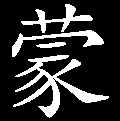
\includegraphics[width=3mm]{../Images/00006}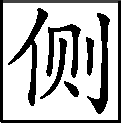
\includegraphics[width=3mm]{../Images/00011}\footnotesize \kaishu 哭成的句子,到今日听了,竟作一场笑话。}黛玉紫鹃听了都笑起来。紫鹃笑道:``这都是素日姑娘念的,难为他怎么记了。''黛玉便令将架摘下来,另挂在月洞窗外的钩上,于是进了屋子,在月洞窗内坐了。吃毕药,只见窗外竹影映入纱来,满屋内阴阴翠润,几簟生凉。黛玉无可释闷,便隔着纱窗调逗鹦哥作戏,又将素日所喜的诗词也教与他念。这且不在话下。

且说薛宝钗来至家中,只见母亲正自梳头呢。一见他来了,便说道:``你大清早起跑来作什么?''宝钗道:``我瞧瞧妈身上好不好。昨儿我去了,不知他可又过来闹了没有?''一面说,一面在他母亲身旁坐了,由不得哭将起来。薛姨妈见他一哭,自己撑不住,也就哭了一场,一面又劝他:``我的儿,你别委曲了,你等我处分他。你要有个好歹,我指望那一个来!''薛蟠在外边听见,连忙跑了过来,对着宝钗,左一个揖,右一个揖,只说:``好妹妹,恕我这一次罢!原是我昨儿吃了酒,回来的晚了,路上撞客着了,来家未醒,不知胡说了什么,连自己也不知道,怨不得你生气。''宝钗原是掩面哭的,听如此说,由不得又好笑了,遂抬头向地下啐了一口,说道:``你不用做这些像生儿。我知道你的心里多嫌我们娘儿两个,是要变着法儿叫我们离了你,你就心净了。''

薛蟠听说,连忙笑道:``妹妹这话从那里说起来的,这样我连立足之地都没了。妹妹从来不是这样多心说歪话的人。''薛姨妈忙又接着道:``你只会听见你妹妹的歪话,难道昨儿晚上你说的那话就应该的不成?当真是你发昏了!''薛蟠道:``妈也不必生气,妹妹也不用烦恼,从今以后我再不同他们一处吃酒闲逛如何?''宝钗笑道:``这不明白过来了!''{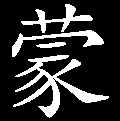
\includegraphics[width=3mm]{../Images/00006}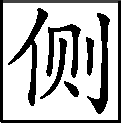
\includegraphics[width=3mm]{../Images/00011}\footnotesize \kaishu 亲生兄妹,形景逼真贴切。}薛姨妈道:``你要有这个横劲,那龙也下蛋了。''薛蟠道:``我若再和他们一处逛,妹妹听见了只管啐我,再叫我畜生,不是人,如何?何苦来,为我一个人,娘儿两个天天操心!妈为我生气还有可恕,若只管叫妹妹为我操心,我更不是人了。如今父亲没了,我不能多孝顺妈多疼妹妹,反教娘生气妹妹烦恼,真连个畜生也不如了。''口里说着,眼睛里禁不起也滚下泪来。{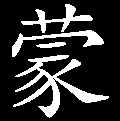
\includegraphics[width=3mm]{../Images/00006}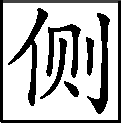
\includegraphics[width=3mm]{../Images/00011}\footnotesize \kaishu 又是一样哭法,不过是情之所至。}

薛姨妈本不哭了,听他一说又勾起伤心来。宝钗勉强笑道:``你闹够了,这会子又招着妈哭起来了。''薛蟠听说,忙收了泪,笑道:``我何曾招妈哭来!罢,罢,罢,丢下这个别提了。叫香菱来倒茶妹妹吃。''宝钗道:``我也不吃茶,等妈洗了手,我们就过去了。''薛蟠道:``妹妹的项圈我瞧瞧,只怕该炸一炸去了。''宝钗道:``黄澄澄的又炸他作什么?''薛蟠又道:``妹妹如今也该添补些衣裳了。要什么颜色花样,告诉我。''宝钗道:``连那些衣服我还没穿遍了,又做什么?''{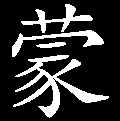
\includegraphics[width=3mm]{../Images/00006}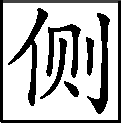
\includegraphics[width=3mm]{../Images/00011}\footnotesize \kaishu 一写骨肉悔过之情,一写本等贞静之女。}一时薛姨妈换了衣裳,拉着宝钗进去,薛蟠方出去了。

这里薛姨妈和宝钗进园来瞧宝玉,到了怡红院中,只见抱厦里外回廊上许多丫鬟老婆站着,便知贾母等都在这里。母女两个进来,大家见过了,只见宝玉躺在榻上。薛姨妈问他可好些。宝玉忙欲欠身,口里答应着``好些'',又说:``只管惊动姨娘、姐姐,我禁不起。''薛姨娘忙扶他睡下,又问他:``想什么,只管告诉我。''宝玉笑道:``我想起来,自然和姨娘要去的。''王夫人又问:``你想什么吃?回来好给你送来的。''宝玉笑道:``也倒不想什么吃,倒是那一回做的那小荷叶儿小莲蓬儿的汤还好些。''凤姐一旁笑道:``听听,口味不算高贵,只是太磨牙了。巴巴的想这个吃了。''贾母便一叠声的叫人做去。凤姐儿笑道:``老祖宗别急,等我想一想这模子谁收着呢。''因回头吩咐个婆子去问管厨房的要去。那婆子去了半天,来回说:``管厨房的说,四副汤模子都交上来了。''凤姐儿听说,想了一想,道:``我记得交上来了,就不记得交给谁了,多半在茶房里。''一面又遣人去问管茶房的,也不曾收。次后还是管金银器皿的送了来。

薛姨妈先接过来瞧时,原来是个小匣子,里面装着四副银模子,都有一尺多长,一寸见方,上面凿着有豆子大小,也有菊花的,也有梅花的,也有莲蓬的,也有菱角的,共有三四十样,打的十分精巧。因笑向贾母王夫人道:``你们府上也都想绝了,吃碗汤还有这些样子。若不说出来,我见这个也不认得这是作什么用的。''凤姐儿也不等人说话,便笑道:``姑妈那里晓得,这是旧年备膳,他们想的法儿。不知弄些什么面印出来,借点新荷叶的清香,全仗着好汤,究竟没意思,谁家常吃他了。那一回呈样的作了一回,他今日怎么想起来了。''说着接了过来,递与个妇人,吩咐厨房里立刻拿几只鸡,另外添了东西,做出十来碗来。王夫人道:``要这些做什么?''凤姐儿笑道:``有个原故:这一宗东西家常不大作,今儿宝兄弟提起来了,单做给他吃,老太太、姑妈、太太都不吃,似乎不大好。不如借势儿弄些大家吃,托赖连我也上个俊儿。''贾母听了,笑道:``猴儿,把你乖的!拿着官中的钱你做人。''说的大家笑了。凤姐也忙笑道:``这不相干。这个小东道我还孝敬的起。''便回头吩咐妇人,``说给厨房里,只管好生添补着做了,在我的账上来领银子。''妇人答应着去了。

宝钗一旁笑道:``我来了这么几年,留神看起来,凤丫头凭他怎么巧,再巧不过老太太去。''贾母听说,便答道:``我如今老了,那里还巧什么。当日我像凤哥儿这么大年纪,比他还来得呢。他如今虽说不如我们,也就算好了,比你姨娘强远了。你姨娘可怜见的,不大说话,和木头似的,在公婆跟前就不大显好。凤儿嘴乖,怎么怨得人疼他。''宝玉笑道:``若这么说,不大说话的就不疼了?''贾母道:``不大说话的又有不大说话的可疼之处,嘴乖的也有一宗可嫌的,倒不如不说话的好。''宝玉笑道:``这就是了。我说大嫂子倒不大说话呢,老太太也是和凤姐姐的一样看待。若是单是会说话的可疼,这些姊妹里头也只是凤姐姐和林妹妹可疼了。''贾母道:``提起姊妹,不是我当着姨太太的面奉承,千真万真,从我们家四个女孩儿算起,全不如宝丫头。''薛姨妈听说,忙笑道:``这话是老太太说偏了。''王夫人忙又笑道:``老太太时常背地里和我说宝丫头好,这倒不是假话。''宝玉勾着贾母原为赞林黛玉的,不想反赞起宝钗来,倒也意出望外,便看着宝钗一笑。宝钗早扭过头去和袭人说话去了。

忽有人来请吃饭,贾母方立起身来,命宝玉好生养着,又把丫头们嘱咐了一回,方扶着凤姐儿,让着薛姨妈,大家出房去了。因问汤好了不曾,又问薛姨妈等:``想什么吃,只管告诉我,我有本事叫凤丫头弄了来咱们吃。''薛姨妈笑道:``老太太也会怄他的。时常他弄了东西孝敬,究竟又吃不了多少。''凤姐儿笑道:``姑妈倒别这样说。我们老祖宗只是嫌人肉酸,若不嫌人肉酸,早已把我还吃了呢。''

一句话没说了,引的贾母众人都哈哈的笑起来。宝玉在房里也撑不住笑了。袭人笑道:``真真的二奶奶的这张嘴怕死人!''宝玉伸手拉着袭人笑道:``你站了这半日,可乏了?''一面说,一面拉他身旁坐了。袭人笑道:``可是又忘了。趁宝姑娘在院子里,你和他说,烦他莺儿来打上几根络子。''宝玉笑道:``亏你提起来。''说着,便仰头向窗外道:``宝姐姐,吃过饭叫莺儿来,烦他打几根络子,可得闲儿?''宝钗听见,回头道:``怎么不得闲儿,一会叫他来就是了。''贾母等尚未听真,都止步问宝钗。宝钗说明了,大家方明白。贾母又说道:``好孩子,叫他来替你兄弟作几根。你要无人使唤,我那里闲着的丫头多呢,你喜欢谁,只管叫了来使唤。''薛姨妈宝钗等都笑道:``只管叫他来作就是了,有什么使唤的去处。他天天也是闲着淘气。''

大家说着,往前迈步正走,忽见史湘云、平儿、香菱等在山石边掐凤仙花呢,见了他们走来,都迎上来了。少顷至园外,王夫人恐贾母乏了,便欲让至上房内坐。贾母也觉腿酸,便点头依允。王夫人便令丫头忙先去铺设坐位。那时赵姨娘推病,只有周姨娘与众婆娘丫头们忙着打帘子,立靠背,铺褥子。贾母扶着凤姐儿进来,与薛姨妈分宾主坐了。薛宝钗史湘云坐在下面。王夫人亲捧了茶奉与贾母,李宫裁奉与薛姨妈。贾母向王夫人道:``让他们小妯娌伏侍,你在那里坐了,好说话儿。''王夫人方向一张小杌子上坐下,便吩咐凤姐儿道:``老太太的饭在这里放,添了东西来。''凤姐儿答应出去,便令人去贾母那边告诉,那边的婆娘忙往外传了,丫头们忙都赶过来。王夫人便令``请姑娘们去''。请了半天,只有探春惜春两个来了;迎春身上不耐烦,不吃饭;林黛玉自不消说,平素十顿饭只好吃五顿,众人也不着意了。少顷饭至,众人调放了桌子。凤姐儿用手巾裹着一把牙箸站在地下,笑道:``老祖宗和姑妈不用让,还听我说就是了。''贾母笑向薛姨妈道:``我们就是这样。''薛姨妈笑着应了。于是凤姐放了四双:上面两双是贾母薛姨妈,两边是薛宝钗史湘云的。王夫人李宫裁等都站在地下看着放菜。凤姐先忙着要干净家伙来,替宝玉拣菜。{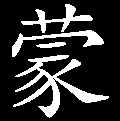
\includegraphics[width=3mm]{../Images/00006}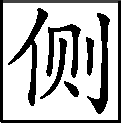
\includegraphics[width=3mm]{../Images/00011}\footnotesize \kaishu 家庭之间,亦复如此。}

少顷,荷叶汤来,贾母看过了。王夫人回头见玉钏儿在那边,便令玉钏与宝玉送去。凤姐道:``他一个人拿不去。''可巧莺儿和喜儿都来了。宝钗知道他们已吃了饭,便向莺儿道:``宝兄弟正叫你去打络子,你们两个一同去罢。''莺儿答应,同着玉钏儿出来。莺儿道:``这么远,怪热的,怎么端了去?''玉钏笑道:``你放心,我自有道理。''说着,便令一个婆子来,将汤饭等物放在一个捧盒里,{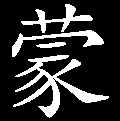
\includegraphics[width=3mm]{../Images/00006}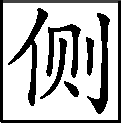
\includegraphics[width=3mm]{../Images/00011}\footnotesize \kaishu 大家气象。}令他端了跟着,他两个却空着手走。一直到了怡红院门内,玉钏儿方接了过来,同莺儿进入宝玉房中。袭人、麝月、秋纹三个人正和宝玉顽笑呢,见他两个来了,都忙起来,笑道:``你两个怎么来的这么碰巧,一齐来了。''一面说,一面接了下来。玉钏便向一张杌子上坐了,莺儿不敢坐下。{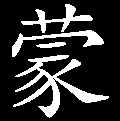
\includegraphics[width=3mm]{../Images/00006}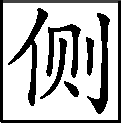
\includegraphics[width=3mm]{../Images/00011}\footnotesize \kaishu 两人不一样写,真是各进其文于后。}袭人便忙端了个脚踏来,{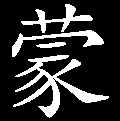
\includegraphics[width=3mm]{../Images/00006}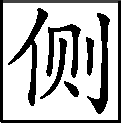
\includegraphics[width=3mm]{../Images/00011}\footnotesize \kaishu 宝卿之婢,自应与众不同。}莺儿还不敢坐。宝玉见莺儿来了,却倒十分欢喜;忽见了玉钏儿,便想到他姐姐金钏儿身上,又是伤心,又是惭愧,便把莺儿丢下,且和玉钏儿说话。袭人见把莺儿不理,恐莺儿没好意思的,{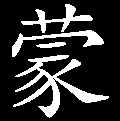
\includegraphics[width=3mm]{../Images/00006}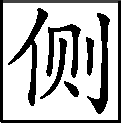
\includegraphics[width=3mm]{../Images/00011}\footnotesize \kaishu 能事者。}又见莺儿不肯坐,便拉了莺儿出来,到那边房里去吃茶说话儿去了。

这里麝月等预备了碗箸来伺候吃饭。宝玉只是不吃,问玉钏儿道:``你母亲身子好?''玉钏儿满脸怒色,正眼也不看宝玉,半日,方说了一个``好''字。宝玉便觉没趣,半日,只得又陪笑问道:{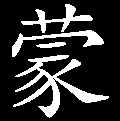
\includegraphics[width=3mm]{../Images/00006}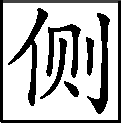
\includegraphics[width=3mm]{../Images/00011}\footnotesize \kaishu 何等涵度。}``谁叫你给我送来的?''玉钏儿道:``不过是奶奶太太们!''宝玉见他还是这样哭丧,便知他是为金钏儿的原故;待要虚心下气磨转他,又见人多,不好下气的,{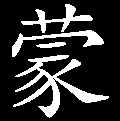
\includegraphics[width=3mm]{../Images/00006}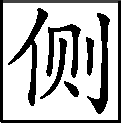
\includegraphics[width=3mm]{../Images/00011}\footnotesize \kaishu 金钏儿如若有知,该何等感激!}因而变尽方法,将人都支出去,然后又陪笑问长问短。

那玉钏儿先虽不悦,只管见宝玉一些性子没有,凭他怎么丧谤,他还是温存和气,自己倒不好意思的了,脸上方有三分喜色。{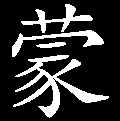
\includegraphics[width=3mm]{../Images/00006}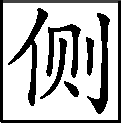
\includegraphics[width=3mm]{../Images/00011}\footnotesize \kaishu 我看到此处,也着实不过意。}宝玉便笑求他:``好姐姐,你把那汤拿了来我尝尝。''玉钏儿道:``我从不会喂人东西,等他们来了再吃。''宝玉笑道:``我不是要你喂我。我因为走不动,你递给我吃了,你好赶早儿回去交代了,你好吃饭的。我只管耽误时候,你岂不饿坏了。你要懒待动,我少不了忍了疼下去取来。''说着便要下床来,扎挣起来,禁不住嗳哟之声。玉钏儿见他这般,忍不住起身说道:``躺下罢!那世里造了来的业,这会子现世现报。教我那一个眼睛看的上!''{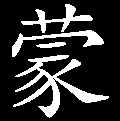
\includegraphics[width=3mm]{../Images/00006}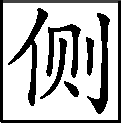
\includegraphics[width=3mm]{../Images/00011}\footnotesize \kaishu 偏于此间写此不情之态,以表白多情之苦。}一面说,一面``哧''的一声又笑了,端过汤来。

宝玉笑道:``好姐姐,你要生气只管在这里生罢,见了老太太、太太可放和气些,若还这样,你就又捱骂了。''玉钏儿道:``吃罢,吃罢!不用和我甜嘴蜜舌的,我可不信这样话!''说着,催宝玉喝了两口汤。宝玉故意说:``不好吃,不吃了。''玉钏儿道:``阿弥陀佛!这还不好吃,什么好吃?''宝玉道:``一点味儿也没有,你不信,尝一尝就知道了。''玉钏儿真就赌气尝了一尝。宝玉笑道:``这可好吃了。''玉钏儿听说,方解过意来,原是宝玉哄他吃一口,便说道:``你既说不好吃,这会子说好吃也不给你吃了。''宝玉只管央求陪笑要吃,{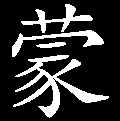
\includegraphics[width=3mm]{../Images/00006}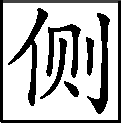
\includegraphics[width=3mm]{../Images/00011}\footnotesize \kaishu 写尽多情人无限委屈柔肠。}玉钏儿又不给他,一面又叫人打发吃饭。

丫头方进来时,忽有人来回话:``傅二爷家的两个嬷嬷来请安,来见二爷。''宝玉听说,便知是通判傅试家的嬷嬷来了。那傅试原是贾政的门生,历年来都赖贾家的名势得意,贾政也着实看待,故与别个门生不同,他那里常遣人来走动。宝玉素习最厌愚男蠢女的,今日却如何又令两个婆子过来?其中原来有个原故:只因那宝玉闻得傅试有个妹子,名唤傅秋芳,也是个琼闺秀玉,常闻人传说才貌俱全,虽自未亲睹,然遐思遥爱之心十分诚敬,不命他们进来,恐薄了傅秋芳,{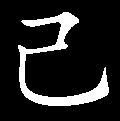
\includegraphics[width=3mm]{../Images/00003}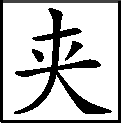
\includegraphics[width=3mm]{../Images/00012}\footnotesize \kaishu 痴想。}因此连忙命让进来。

那傅试原是暴发的,因傅秋芳有几分姿色,聪明过人,那傅试安心仗着妹妹要与豪门贵族结姻,不肯轻易许人,所以耽误到如今。目今傅秋芳年已二十三岁,尚未许人。争奈那些豪门贵族又嫌他穷酸,根基浅薄,不肯求配。{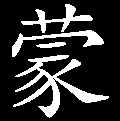
\includegraphics[width=3mm]{../Images/00006}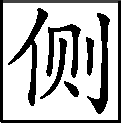
\includegraphics[width=3mm]{../Images/00011}\footnotesize \kaishu 大抵诸色非情不生,非情不合。情之表见于爱,爱众则心无定象,心不定则诸幻丛生,诸魔蜂起,则汲汲乎流于无情。此宝玉之多情而不情之案,凡我同人其留意!}那傅试与贾家亲密,也自有一段心事。今日遣来的两个婆子偏生是极无知识的,闻得宝玉要见,进来只刚问了好,说了没两句话。那玉钏见生人来,也不和宝玉厮闹了,手里端着汤只顾听话。宝玉又只顾和婆子说话,一面吃饭,一面伸手去要汤。两个人的眼睛都看着人,不想伸猛了手,便将碗碰翻,将汤泼了宝玉手上。玉钏儿倒不曾烫着,唬了一跳,忙笑了,``这是怎么说!''慌的丫头们忙上来接碗。宝玉自己烫了手倒不觉的,却只管问玉钏儿:``烫了那里了?疼不疼?''{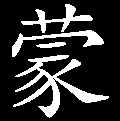
\includegraphics[width=3mm]{../Images/00006}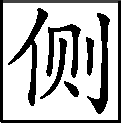
\includegraphics[width=3mm]{../Images/00011}\footnotesize \kaishu 多情人每于苦恼时不自觉,反说彼家苦恼。爱之至、惜之深之故也。}玉钏儿和众人都笑了。玉钏儿道:``你自己烫了,只管问我。''宝玉听说,方觉自己烫了。众人上来连忙收拾。宝玉也不吃饭了,洗手吃茶,又和那两个婆子说了两句话。然后两个婆子告辞出去,晴雯等送至桥边方回。

那两个婆子见没人了,一行走,一行谈论。这一个笑道:``怪道有人说他家宝玉是外像好里头糊涂,中看不中吃的,果然有些呆气。他自己烫了手,倒问人疼不疼,这可不是个呆子?''那一个又笑道:``我前一回来,听见他家里许多人抱怨,千真万真的有些呆气。大雨淋的水鸡似的,他反告诉别人:`下雨了,快避雨去罢。'你说可笑不可笑?时常没人在跟前,就自哭自笑的;看见燕子,就和燕子说话;河里看见了鱼,就和鱼说话;见了星星月亮,不是长吁短叹,就是咕咕哝哝的。且是连一点刚性也没有,连那些毛丫头的气都受的。爱惜东西,连个线头儿都是好的;糟踏起来,那怕值千值万的都不管了。''{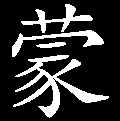
\includegraphics[width=3mm]{../Images/00006}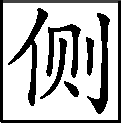
\includegraphics[width=3mm]{../Images/00011}\footnotesize \kaishu 如人饮水,冷暖自知。其中深意味,岂能持告君?}两个人一面说,一面走出园来,辞别诸人回去,不在话下。{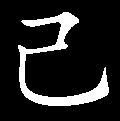
\includegraphics[width=3mm]{../Images/00003}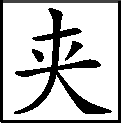
\includegraphics[width=3mm]{../Images/00012}\footnotesize \kaishu 宝玉之为人,非此一论,亦描写不尽;宝玉之不肖,非此一鄙,亦形容不到。试问作者是丑宝玉乎,是赞宝玉乎?试问观者是喜宝玉乎,是恶宝玉乎?}

如今且说袭人见人去了,便携了莺儿过来,问宝玉打什么络子。宝玉笑向莺儿道:``才只顾说话,就忘了你。烦你来不为别的,却为替我打几根络子。''莺儿道:``装什么的络子?''宝玉见问,便笑道:``不管装什么的,你都每样打几个罢。''{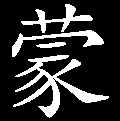
\includegraphics[width=3mm]{../Images/00006}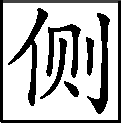
\includegraphics[width=3mm]{../Images/00011}\footnotesize \kaishu 富家子弟每多有如是语,只不自觉耳。}莺儿拍手笑道:``这还了得!要这样,十年也打不完了。''宝玉笑道:``好姐姐,你闲着也没事,都替我打了罢。''袭人笑道:``那里一时都打得完,如今先拣要紧的打两个罢。''莺儿道:``什么要紧,不过是扇子、香坠儿、汗巾子。''宝玉道:``汗巾子就好。''莺儿道:``汗巾子是什么颜色的?''宝玉道:``大红的。''莺儿道:``大红的须是黑络子才好看的,或是石青的才压的住颜色。''宝玉道:``松花色配什么?''莺儿道:``松花配桃红。''宝玉笑道:``这才娇艳。再要雅淡之中带些娇艳。''莺儿道:``葱绿柳黄是我最爱的。''宝玉道:``也罢了,也打一条桃红,再打一条葱绿。''莺儿道:``什么花样呢?''宝玉道:``共有几样花样?''莺儿道:``一炷香、朝天凳、象眼块、方胜、连环、梅花、柳叶。''宝玉道:``前儿你替三姑娘打的那花样是什么?''莺儿道:``那是攒心梅花。''宝玉道:``就是那样好。''一面说,一面叫袭人,刚拿了线来,窗外婆子说``姑娘们的饭都有了。''宝玉道:``你们吃饭去,快吃了来罢。''袭人笑道:``有客在这里,我们怎好去的!''{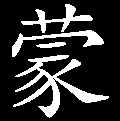
\includegraphics[width=3mm]{../Images/00006}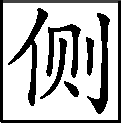
\includegraphics[width=3mm]{../Images/00011}\footnotesize \kaishu 人情物理,一丝不乱。}莺儿一面理线,一面笑道:``这话又打那里说起,正经快吃了来罢。''袭人等听说方去了,只留下两个小丫头听呼唤。

宝玉一面看莺儿打络子,一面说闲话,因问他:``十几岁了?''莺儿手里打着,一面答话说:``十六岁了。''宝玉道:``你本姓什么?''莺儿道:``姓黄。''宝玉笑道:``这个名姓倒对了,果然是个黄莺儿。''莺儿笑道:``我的名字本来是两个字,叫作金莺。姑娘嫌拗口,就单叫莺儿,如今就叫开了。''宝玉道:``宝姐姐也算疼你了。明儿宝姐姐出阁,少不得是你跟去了。''莺儿抿嘴一笑。宝玉笑道:``我常常和袭人说,明儿不知那一个有福的消受你们主子奴才两个呢。''{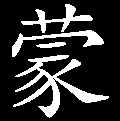
\includegraphics[width=3mm]{../Images/00006}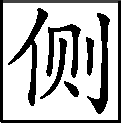
\includegraphics[width=3mm]{../Images/00011}\footnotesize \kaishu 是有心?是无心?}莺儿笑道:``你还不知道,我们姑娘有几样世人都没有的好处呢,模样儿还在次。''宝玉见莺儿娇憨婉转,语笑如痴,早不胜其情了,那更提起宝钗来!便问他道:``好处在那里?好姐姐,细细告诉我听。''莺儿笑道:``我告诉你,你可不许又告诉他去。''{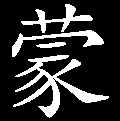
\includegraphics[width=3mm]{../Images/00006}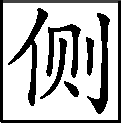
\includegraphics[width=3mm]{../Images/00011}\footnotesize \kaishu 闺房闲话,着实幽韵。}宝玉笑道:``这个自然的。''正说着,只听外头说道:``怎么这样静悄悄的!''二人回头看时,不是别人,正是宝钗来了。宝玉忙让坐。宝钗坐了,因问莺儿``打什么呢?''一面问,一面向他手里去瞧,才打了半截。宝钗笑道:``这有什么趣儿,倒不如打个络子把玉络上呢。''一句话提醒了宝玉,便拍手笑道:``倒是姐姐说得是,我就忘了。只是配个什么颜色才好?''宝钗道:``若用杂色断然使不得,大红又犯了色,黄的又不起眼,黑的又过暗。等我想个法儿:把那金线拿来,配着黑珠儿线,一根一根的拈上,打成络子,这才好看。''

宝玉听说,喜之不尽,一叠声便叫袭人来取金线。正值袭人端了两碗菜走进来,告诉宝玉道:``今儿奇怪,才刚太太打发人给我送了两碗菜来。''宝玉笑道:``必定是今儿菜多,送来给你们大家吃的。''袭人道:``不是,指名给我送来的,还不叫我过去磕头。这可是奇了。''宝钗笑道:``给你的,你就吃了,这有什么可猜疑的。''袭人笑道:``从来没有的事,倒叫我不好意思的。''宝钗抿嘴一笑,说道:``这就不好意思了?{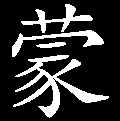
\includegraphics[width=3mm]{../Images/00006}\includegraphics[width=3mm]{../Images/00011}\footnotesize \kaishu 宝{(玉)}{[}钗{]}之慧性灵心。}明儿比这个更叫你不好意思的还有呢。''袭人听了话内有因,素知宝钗不是轻嘴薄舌奚落人的,自己方想起上日王夫人的意思来,便不再提,将菜与宝玉看了,说:``洗了手来拿线。''说毕,便一直的出去了。吃过饭,洗了手,进来拿金线与莺儿打络子。此时宝钗早被薛蟠遣人来请出去了。

这里宝玉正看着打络子,忽见邢夫人那边遣了两个丫鬟送了两样果子来与他吃,问他``可走得了?若走得动,叫哥儿明儿过来散散心,太太着实记挂着呢。''宝玉忙道:``若走得了,必请太太的安去。疼的比先好些,请太太放心罢。''一面叫他两个坐下,一面又叫秋纹来,把才拿来的那果子拿一半送与林姑娘去。秋纹答应了,刚欲去时,只听黛玉在院内说话,宝玉忙叫:``快请。''要知端的,且听下回分解。

{\includegraphics[width=3mm]{../Images/00005}总评:此回是以情说法,警醒世人。黛玉因情凝思默度,忘其有身,忘其有病;而宝玉千屈万折,因情忘其尊卑,忘其痛苦,并忘其性情。爱河之深无底,何可泛滥,一溺其中,非死不止。且泛爱者不专,新旧叠增,岂能尽了?其多情之心不能不流于无情之地。究其立意,倏忽千里而自不觉。诚可悲乎!}
